\documentclass[a4paper,11pt]{article}
\usepackage[utf8]{inputenc}
\usepackage[italian]{babel}
%\usepackage[top=3 cm, bottom=3.5 cm, left=2.5 cm, right=2.5 cm]{geometry}
\usepackage{siunitx}
\usepackage{fancyhdr}
\usepackage{amsthm}
\usepackage{amsmath}
\usepackage{amssymb}
\usepackage{graphicx}
\usepackage{float}
\usepackage{braket}
\usepackage{tikz}
\usetikzlibrary{decorations}
\usetikzlibrary{er}
\graphicspath{{./img/}}

\author{Ruggero Lot \\ ruggero90@gmail.com \\ fisica della materia \\}
\title{Esame di MBS}
\begin{document}
	\maketitle
	\paragraph{Problema:} % (fold)
	\label{par:problema}
		Si consideri un cristallo LJ con un interstiziale: ovvero una struttura
		FCC di N siti cristallini occupati da N+1 atomi, l' N+1-mo trovandosi in
		un sito non FCC. Si ponga l'atomo addizionale in modo da massimizzare la
		distanza dai primi vicini (il cristallo sarà sotto stress, si calcoli la
		struttura di equilibrio usando uno Steepest Descent).\\
		L'obiettivo è di calcolare il coefficiente di autodiffusione D, il quale,
		visto che il cristallo perfetto praticamente non diffonde, sarà dovuto 
		interamente all'atomo addizionale. Può essere che per vedere una diffusione
		apprezzabile sia necessario avvicinarsi alla T di fusione, facendo
		attenzione a verificare che il sistema rimanga solido (calcoli affini
		nello stato liquido possono essere d'aiuto). A questo fine può essere
		utile partire da T relativamente basse per poi eseguire simulazioni a T
		via via più alte, ogni volta partendo dallo stato finale della simulazione
		precedente.\\
		Eseguire un fit di $D(T)$ seguendo la relazione di Arrhenius
		\begin{equation*}
			D = D_0 e^{\frac{Q}{kT}}. 
		\end{equation*}
		Stimare la dipendenza di D da N per almeno una T.
	% paragraph problema (end)
	\newpage
	\tableofcontents
	\newpage
	\section{Software per la creazione del Sample} % (fold)
	\label{sec:software_per_la_creazione_del_sample}
		Il software ``starting\_positions'' è stato generato allo scopo di poter 
		generare un campione sul quale andare poi ad eseguire simulazioni per
		raccogliere dati sul comportamento delle particelle.\\
		Il campione generato attraverso questo strumento consiste in un reticolo
		FCC (di passo reticolare a piacere) con un atomo interstiziale(se 
		richiesto) contenuto in una scatola cubica (di lato l) e pronto per
		essere utilizzato in algoritmi capaci di implementare le condizioni 
		periodiche al contorno.\\
		Il software consta di 2 algoritmi: il primo è quello di posizionamento 
		delle particelle all'interno della scatola, operazione che viene svolta
		in maniera sequenziale inserendo i 4 atomi per ogni cella unitaria nelle 
		posizioni FCC con la base:
		\begin{align}
			\mathbf a_1  &= a(0,0,0) & 
			\mathbf a_2  &= a(0,0.5,0.5) &
			\mathbf a_3  &= a(0.5,0,0.5) 
		\end{align}
		scartando eventuali atomi esterni alla scatola o doppi a causa delle pbc.\\
		Il secondo invece si occupa di portare il sistema, se sotto stress, ad uno 
		stato di equilibrio. Per risolvere questo problema è stato utilizzato uno 
		Steepest Descent che viene implementato nel seguente modo:
		\begin{center}
			\begin{tikzpicture}
				[text depth=1pt,
				every attribute/.style={fill=black!20,draw=black},
				every entity/.style={fill=blue!20,draw=blue,thick},
				every relationship/.style={fill=orange!20,draw=orange,thick,aspect=1.5}]
				
				\node[entity] (F) at (-3,0) {Rifiuto la mossa} 
					child {node [entity]{Gradiente} child {node [entity]{step}}};
				
				\node[entity] (F) at (-3,0) {Rifiuto la mossa} 
					child {node [entity]{Gradiente} child {node [entity]{step}}};
				\node[relationship] (T) at (0,-2) {$\Delta E < \epsilon$}
					child {node [entity]{Step} child {node [entity]{E = E + 1}}};
	
				\node[relationship]	at (0,0) {file.py} 
					edge (F) 
					edge (T);
			\end{tikzpicture}	
	    \end{center}
	    Questo metodo non è molto rapido ma ci permette di ottenere comunque
	    risultati ragionevoli in tempi contenuti.
	    Nota importante, è stata inserita una normalizzazione del vettore di discesa
	    per evitare, soprattutto nelle fasi iniziali dove il vettore gradiente ha 
	    modulo molto grande, salti spaziali delle particelle privi di significato fisico.
	% section software_per_la_creazione_del_sample (end)
	\subsection{Dati ottenuti} % (fold)
	\label{sub:dati_ottenuti}
		questo primo programma è stato fatto eseguire con dei valori numerici 
		pensati in modo tale da garantire immediatamente una situazione di stabilità
		del sistema eccezion fatta per la particella interstiziale che viene posizionata in maniera del tutto casule all'interno della scatola.
		\paragraph{Cella unitaria e scatola di simulazione\\} % (fold)
		\label{par:cella_unitaria_e_scatola_di_simulazione}
			Per la cella unitaria è stata valutata la situazione di maggior 
			stabilità: il potenziale di LJ
			\begin{equation}
				U(\mathbf{r}_{ij})= 4 \epsilon \left(\left(\frac{\sigma}{\mathbf{r}_{ij}}\right)^{12}\
				-\left(\frac{\sigma}{\mathbf{r}_{ij}}\right)^6\right)
			\end{equation}
			ha un minimo in:
			\begin{equation}
				\left|\mathbf{r}_{ij}\right| = 2^{\frac{1}{6}} \sigma
				\approx 2.12 \sigma
			\end{equation}
			pertanto il lato della cella FCC risulta essere, ponendo $\sigma = 1$:
			\begin{equation}
				l = \frac{2^{\frac{1}{6}+1}}{\sqrt{2}} \approx 1.59
			\end{equation}
			per la nostra scatola cubica sono stati scelti valori di lato pari a 
			$2l$, $3l$, $4l$, $5l$ che sono capaci di contenere rispettivamente: 
			$32$, $108$, $256$, $512$ particelle
		% paragraph cella_unitaria_e_scatola_di_simulazione (end)
		\paragraph{Evoluzione dell'energia durante lo Steepest Descent\\} % (fold)
		\label{par:evoluzione_dell_energia_durante_lo_steepest_descent}
			\`E comune osservare in tutti i grafici come l'energia sia molto
			elevata all'inizio e tenda rapidamente ad un valore molto piccolo per
			poi mantenersi quasi stabile.\\
			Questo è dovuto al fatto che la particella aggiunta in maniera 
			completamente casuale si trova quasi sempre vicino ad un altra 
			particella e il potenziale di ordine 12 fa si che anche piccoli
			spostamenti (i primi steps) causino grandi variazioni di energia;
			raggiunta in seguito una configurazione stabile questo 
			fenomeno sparisce.\\
			

			\begin{figure}[H]
					\centering
					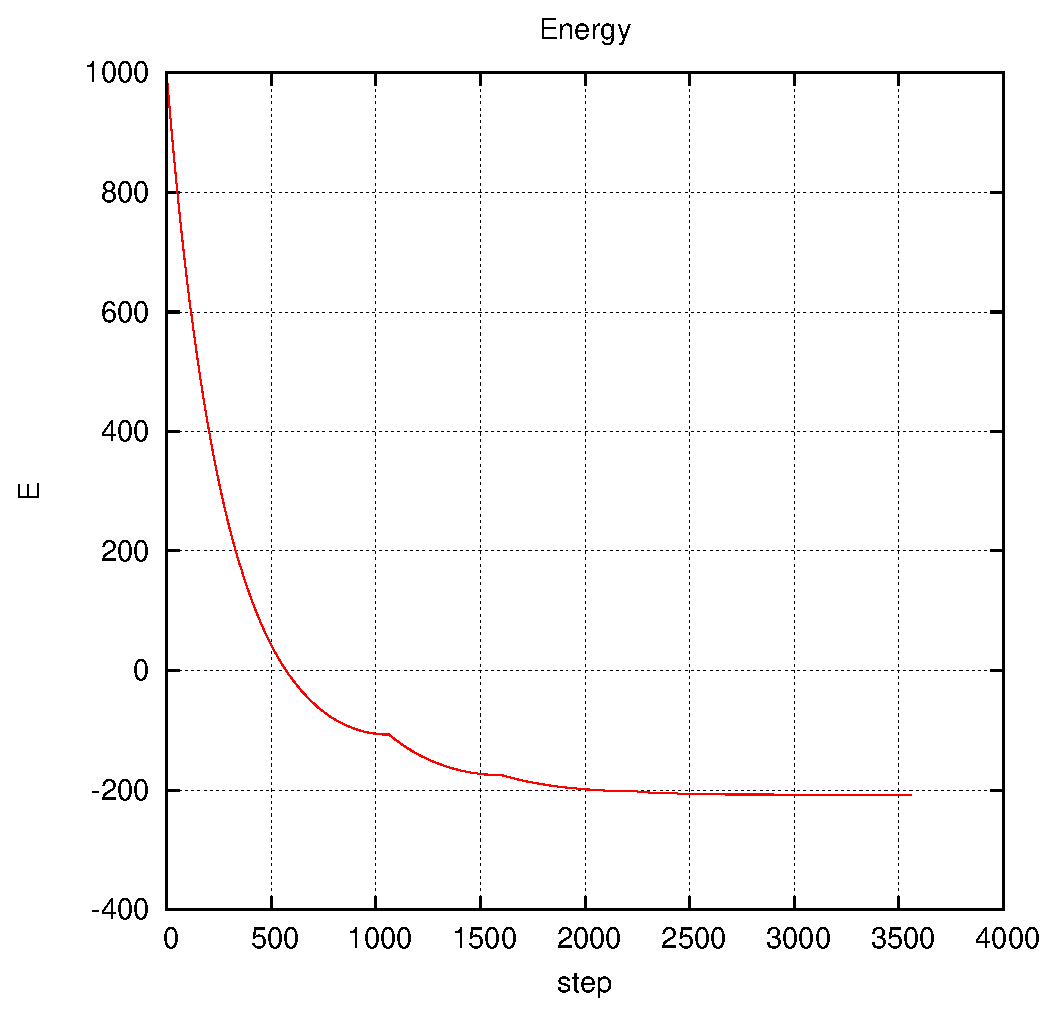
\includegraphics[scale = 0.7]{E_SD_32.eps}
					\caption{andameto dell'energia durante lo Steepest Descent per il campione composto da 32 particelle. Si notano chiaramente i cambi di direzione del gradiente ed si osserva come la convergenza non impieghi molti step}
					\label{fig:SD_32}
				\end{figure}	
		% paragraph evoluzione_dell_energia_durante_lo_steepest_descent (end)
	% subsection dati_ottenuti (end)
\end{document}